% Load footnote extensions before hyperref to keep package definitions compatible.
\AddToHook{package/hyperref/before}{\RequirePackage{scrextend}}
\documentclass[bp]{FEIstyle}
\usepackage{tikz}
\usetikzlibrary{arrows.meta,calc,decorations.pathreplacing,fit,positioning,shapes.geometric}

% Author of the thesis
\FEIauthor{Postaichuk Pavlo}

% Evidence number
\FEIregNr{FEI-xxxx-xxxx}

% Title
\FEItitle{Blockchain analýza}
\FEItitleEn{Blockchain analysis}

% Date
\FEIdate{--}{--}{2026}

% Keywords
\FEIkeywords{Bitcoin, Elliptic Bitcoin Dataset, analýza blockchainu, únik informácií, grafové neurónové siete}

\FEIkeywordsEn{Bitcoin, Elliptic Bitcoin Dataset, blockchain analysis, data leakage, graph neural networks}

% Further details
\FEIstudyProgramme{Aplikovaná informatika}
\FEIstudyProgrammeEn{Applied Informatics}

\FEIstudyField{informatika}
\FEIstudyFieldEn{Computer Science}

\FEItrainingWorkplace{Ústav informatiky a matematiky FEI STU}
\FEItrainingWorkplaceEn{Institute of Computer Science and Mathematics, FEI STU}

% Supervisor
\FEIsupervisor{prof. Ing. Pavol Zajac, PhD.}


% TODO: nahradiť ukážkové skratky vlastnými a potom zapnúť slovník.
%\FEIglossaries{includes/glossary}

%\FEIlistOfGlossaries
%\FEImanualListOfGlossaries{includes/manual_glossary}

% Bibliography database file
\addbibresource{includes/bibliography.bib}

\begin{document}

%%%%%%%%%%%%%%%%%%
%%              %%
%% FRONT MATTER %%
%%              %%
%%%%%%%%%%%%%%%%%%
\frontmatter

\FEIpdfInfo
\FEIcover
\FEItitlePage
% TODO: vložiť oficiálne zadanie z AIS namiesto ukážkového PDF.
%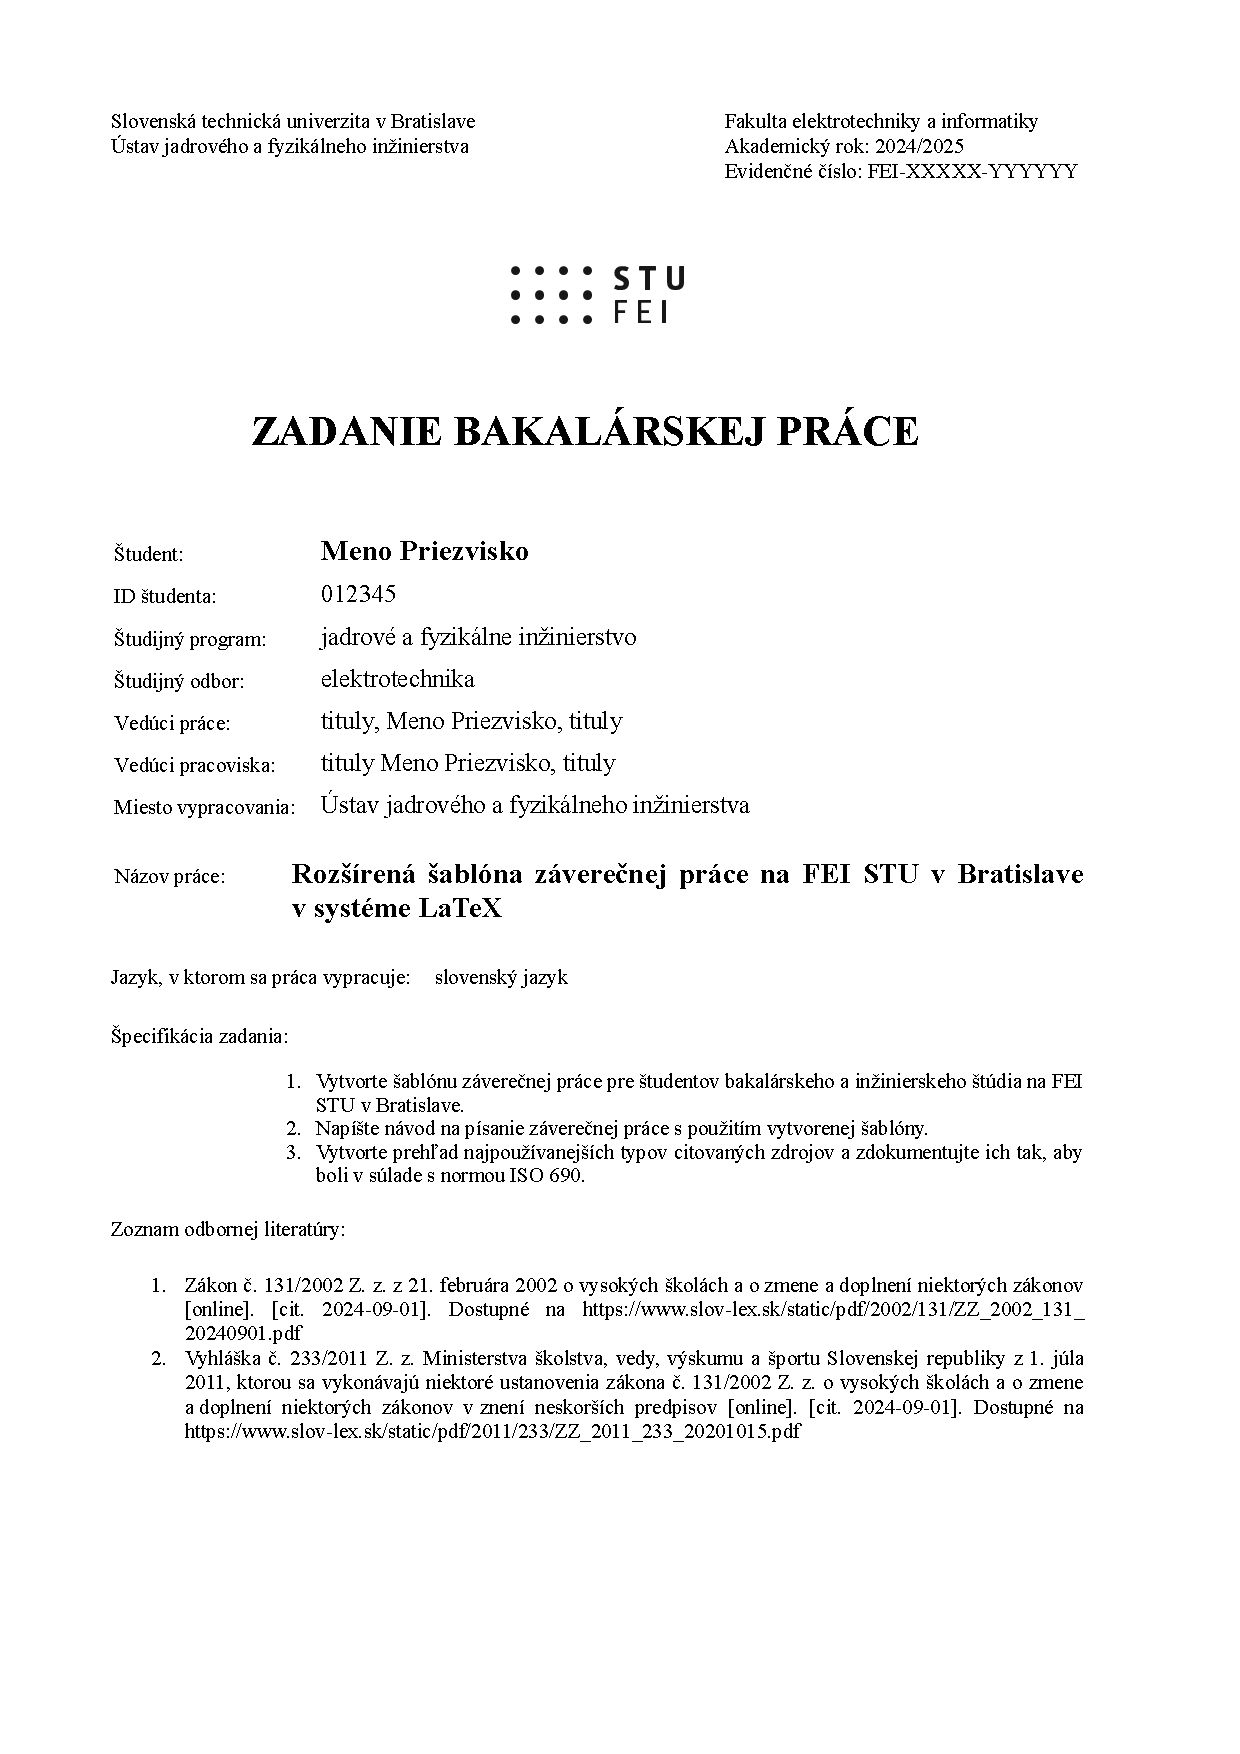
\includepdf[pages=-]{includes/assignment.pdf}
% TODO: doplniť poďakovanie, ak ho autor chce zaradiť.
%\FEIthanks{includes/thanks}
\FEIabstract{includes/abstract}
\FEIabstractEn{includes/abstractEN}
\FEIcontent
\FEIlistOfFiguresAndTables

%% List of units and abbreviations
%%
%% Choose the method of typesetting the list of
%% units and abbreviations.
%% Uncomment only one of the two lines below!

%% METHOD 1:
%% ---------
%% Automatically generated and sorted list of
%% abbreviations with hyperlinks from the text.
%% Edit includes/glossary.tex.
%\FEIlistOfGlossaries
%% METHOD 2:
%% ---------
%% Manual list -- must be manually filled and sorted,
%% does not make hyperlinks from the text.
%% Edit includes/manual_glossary.tex.
\FEImanualListOfGlossaries{includes/manual_glossary}

%% Lists of algorithms and listings
%\FEIlistOfAlgorithms
%\FEIlistOfListings

%%%%%%%%%%%%%%%%%
%%             %%
%% MAIN MATTER %%
%%             %%
%%%%%%%%%%%%%%%%%
\mainmatter

\FEIintroduction{includes/introduction}
\FEIcore{includes/core}
\FEIconclusion{includes/conclusion}

%% Uncomment only if the document is writen in english
%\FEIresume{includes/resume}

%%%%%%%%%%%%%%%%%%
%%              %%
%% Bibliography %%
%%              %%
%%%%%%%%%%%%%%%%%%
\FEIbibliography
%% AI Declaration
% TODO: pravdivo uviesť použitie AI podľa pravidiel STU.
%\FEIaiDeclaration{includes/ai_declaration}

%%%%%%%%%%%%%%%%%%
%%              %%
%% BACK MATTER  %%
%%              %%
%%%%%%%%%%%%%%%%%%
\backmatter

%% Attachment A
%\FEIappendix{Algoritmus\label{att:algorithms}}{includes/attachmentA}

%% Attachment B
%\FEIappendix{Výpis dlhého kódu\label{att:listings}}{includes/attachmentB}

%% Attachment C
%\FEIappendix{Slovníček pojmov\label{att:dictionary}}{includes/attachmentC}

%% Attachement D
%\FEIappendix{Súborová štruktúra projektu\label{att:files}}{includes/attachmentD}


\end{document}
